% PREAMBLE TO DOCUMENT
\documentclass[10pt,twoside,titlepage]{article}% Type of document
  	\usepackage{graphicx}		% Graphics package
  	\usepackage{subfig}		    	% Allows for subfigures	
	\usepackage{wrapfig}			% Allows figure inline with text
 	\usepackage{fancyvrb}		% Verbatim package for MATLAB code
	\usepackage{multicol}			% Multiple column enviroment
	\usepackage{textcomp}		% Money symbols used from this package
 	\usepackage{colortbl} 			% Allows colors in excel tables
 	\usepackage{natbib,multibib}	% Author-Date system
 	\usepackage{amsmath}       % Utilizes AMS-Latex package
 	\usepackage{float}				% Advanced float options
 	\usepackage{afterpage}		% Improving \clearpage
 	\usepackage{flafter}				% Forces floats after references
 	\usepackage{array}				% Extension for tabular environment
 	\usepackage{rotating}			% Allows for sideways or landscape floats
 	\usepackage{tabulary}			% Allows for establishing total table width
 	\usepackage{longtable}		
 	\usepackage[table]{xcolor}% Enables addition of color rows/columns in tables
 	\usepackage{color}				% Allows user to define custom colors
%  	\usepackage{supertabular,xtab}				% Allows for mutliple page tables
 	\usepackage{multirow}		% Enables multiple row items in tables
	\usepackage{calc}					% Allows for computations to be made
	\usepackage{slashbox}		% Adds slashed box option for tables
	\usepackage{soul}					% Inproves underlines
	\usepackage[below]{placeins}			% Allows \FloatBarrier to be used
	\usepackage{listings}		    % Used for code and daily log display
	\usepackage{ifthen}

	\usepackage{ragged2e}
	
%  	\usepackage{setspace}\onehalfspacing 			% Allows for spacing variations
	\usepackage{indentfirst}% Indents the first paragraph of sections
	\usepackage{titlesec,titletoc}
	
% Set margins	
% 	\usepackage[paper=letterpaper, top=1in, bottom=1.75in, outer=0.75in, inner=0.75in, bindingoffset=1.875in,footskip=3ex]{geometry}
	\usepackage[papersize={7in,10in}, top=1in, bottom=0.75in, outer=0.75in, inner=0.75in, bindingoffset=0.25in]{geometry}
	
\definecolor{darkgreen}{rgb}{0,0.4,0}
\lstdefinestyle{inline}{frame=lines, xleftmargin=0pt, numbers=none, basicstyle=\scriptsize}
\lstdefinestyle{figure}{numbers=left, frame=shadowbox, numberstyle={\tiny} ,numbersep=5pt, xleftmargin=2.5em, language=Matlab, basicstyle=\scriptsize, stringstyle=\ttfamily, keywordstyle=\color{blue}, commentstyle=\color{darkgreen}, breaklines=true, breakatwhitespace=false} 
\lstdefinestyle{file}{numbers=left, frame=single, numberstyle={\tiny} ,numbersep=5pt, xleftmargin=2.5em, language=Matlab, basicstyle=\tiny, stringstyle=\ttfamily, keywordstyle=\color{blue}, commentstyle=\color{darkgreen}, breaklines=true, breakatwhitespace=false} 

\title{Thermal Model Software User Manual}\label{apx:thermal}
\author{Andrew E. Slaughter}

\begin{document}
\maketitle
\tableofcontents\clearpage
\section{Introduction}
This document details the implementation of the thermal model software developed and divided into four main sections.  The first section explains how to install and report problems with the software. Section \ref{TM:sec:basic} explains the basic operation of the thermal software.  Section \ref{TM:sec:spread} presents an interface that links the thermal model with Microsoft Excel, allowing inputs to be easily modified.  Figure \ref{TM:fig:flow} contains a flow chart demonstrating how the various functions detailed in the first two sections (\ref{TM:sec:basic} and \ref{TM:sec:spread}) interact. Finally, in Section \ref{TM:sec:gui}, a complete graphical user interface is briefly presented that operates as a stand-alone Windows application.

A few notational conventions are utilized throughout this user manual:
\begin{itemize}
\item Monospaced typeface indicates a MATLAB m-file, function, or variable (e.g., \texttt{sobol.m}).
\item MATLAB code is provided in figure windows (e.g., Figure \ref{SA:fig:fang} when referenced many times).
\item MATLAB code is also presented in-line with the text as:
\begin{lstlisting}[style=inline]
>> 2+2
ans = 4 
>>
\end{lstlisting}\vspace*{0pt}
\end{itemize}

\begin{figure}[ht!]\centering
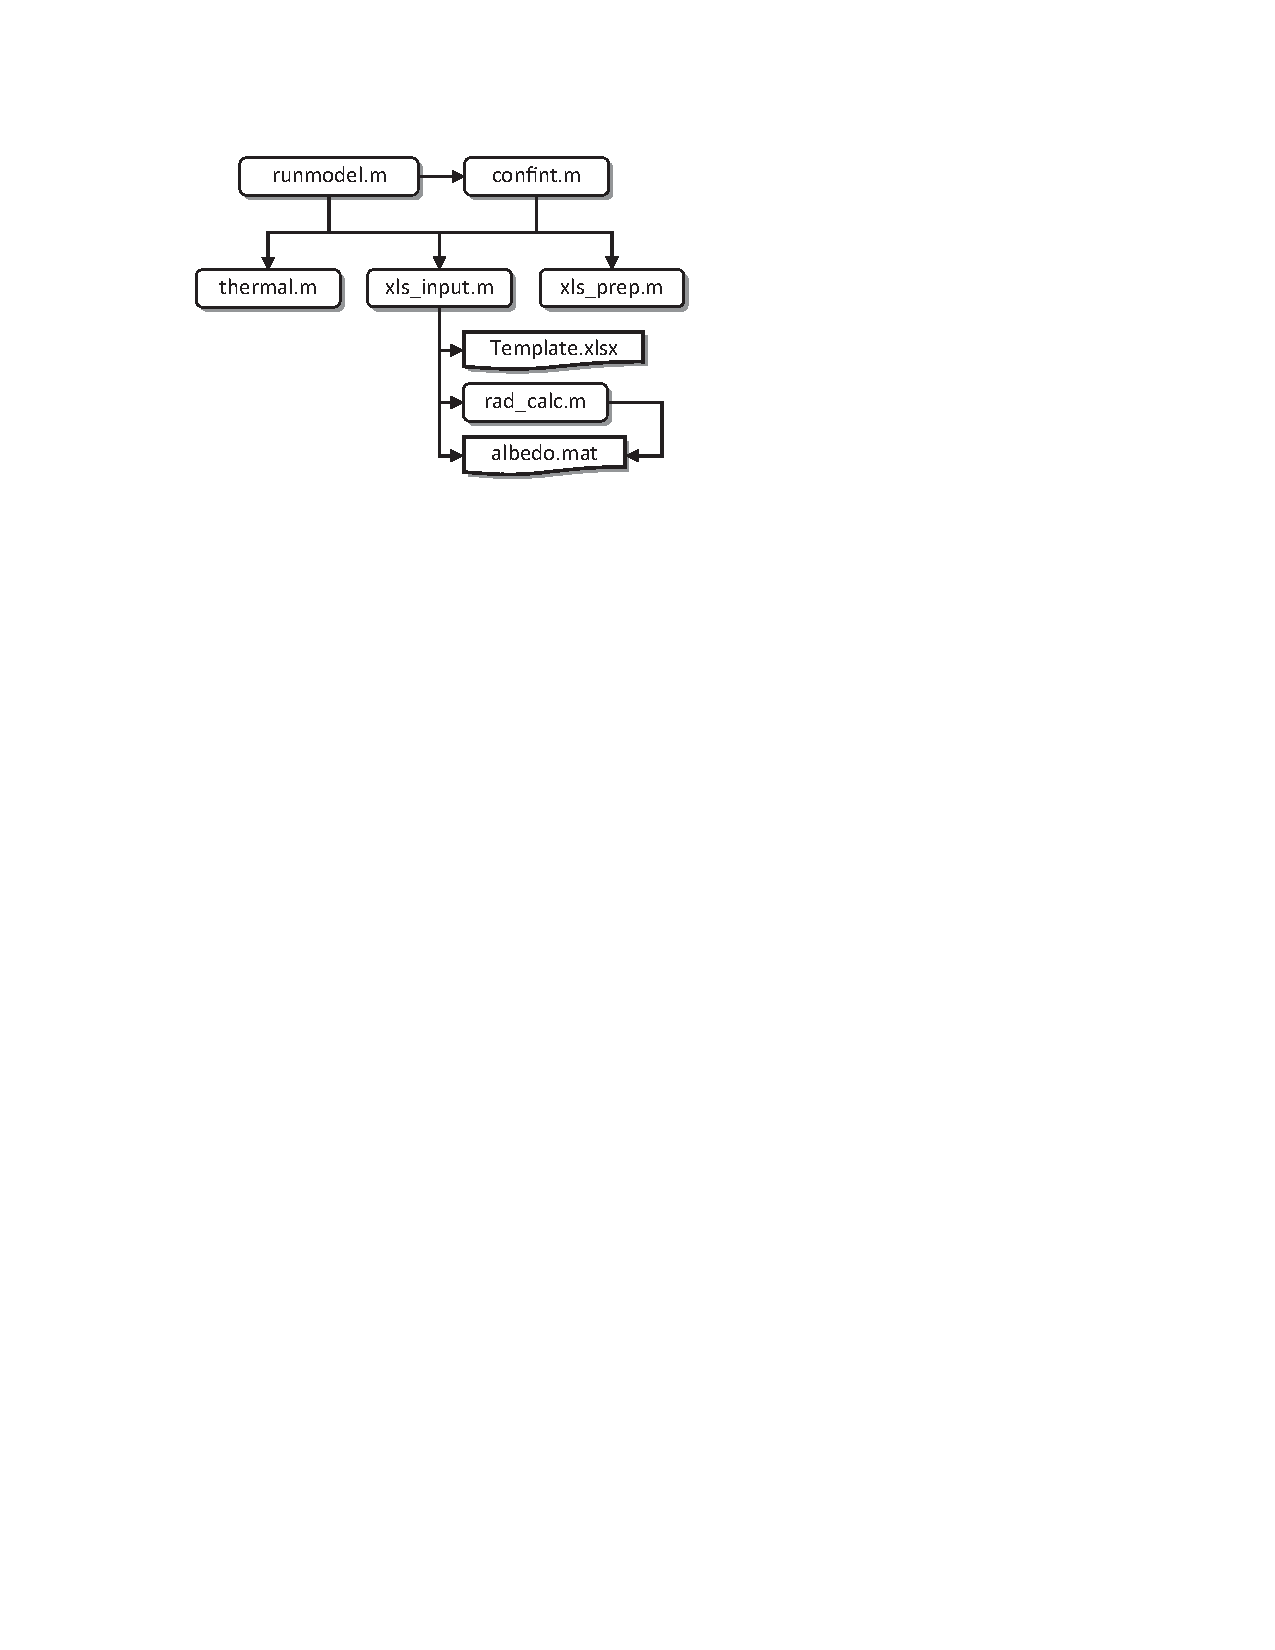
\includegraphics{figures/flow.pdf}
\caption{Flow chart demonstrating how the various functions discussed interact.}
\label{TM:fig:flow}
\end{figure}

\section{Installation and Bug Reporting}

\end{document}